
    \centering
    % ESTA LÍNEA es la que crea el PDF en la carpeta /tikz
    \tikzsetnextfilename{ejercicio27_figura} 
    
    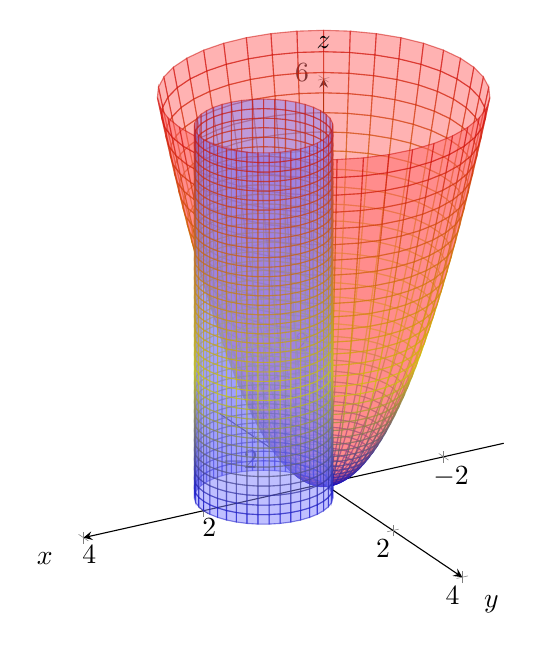
\begin{tikzpicture}
        \begin{axis}[
            view={150}{25}, % Cámara: eje x hacia adelante/izq, eje y hacia la derecha
            width=10cm,
            height=10cm,
            grid=major,
            xmin=-3, xmax=4, % Ajusté un poco los ejes para que se vea mejor
            ymin=-3, ymax=4,
            zmin=0, zmax=6,
            axis lines=center,
            xlabel={$x$},
            ylabel={$y$},
            zlabel={$z$},
            % Estos 3 comandos evitan que las letras queden flotando en cualquier lado
            every axis x label/.style={at={(ticklabel* cs:1.05)},anchor=north east},
            every axis y label/.style={at={(ticklabel* cs:1.05)},anchor=north west},
            every axis z label/.style={at={(ticklabel* cs:1.05)},anchor=south},
        ]

        % Paraboloide z = x^2 + y^2 (Rojo)
        \addplot3[
            surf,
            domain=0:360,
            y domain=0:2.4,
            samples=40,
            color=red!60,
            opacity=0.5,
            z buffer=sort, % Esto arregla el renderizado de la transparencia
        ]
        ({y*cos(x)}, {y*sin(x)}, {y^2});

        % Cilindro (x-1)^2 + y^2 = 1 (Azul)
        \addplot3[
            surf,
            domain=0:360,
            y domain=0:5.5,
            samples=40,
            color=blue!50,
            opacity=0.5,
            z buffer=sort, % Esto arregla el renderizado de la transparencia
        ]
        ({1+cos(x)}, {sin(x)}, {y});

        \end{axis}
    \end{tikzpicture}
    \caption{Representación de la región $W$. \href{https://www.geogebra.org/classic/q6ujp7ap}{Ver en GeoGebra}}
